\documentclass[11pt]{article}
\usepackage[margin=1in]{geometry}
\usepackage{graphicx}
\usepackage{float}
\usepackage{hyperref}
\usepackage{caption}
\captionsetup[figure]{font=small}
\setlength{\parskip}{6pt}
\setlength{\parindent}{0pt}

\title{WebSim Software Engineering Diagrams}
\author{Auto-generated from project documentation}
\date{\today}

\begin{document}
\maketitle

This PDF exports the core engineering diagrams for \texttt{WebSim}.

\section*{1. System Architecture (Component / Container)}
\begin{figure}[H]
  \centering
  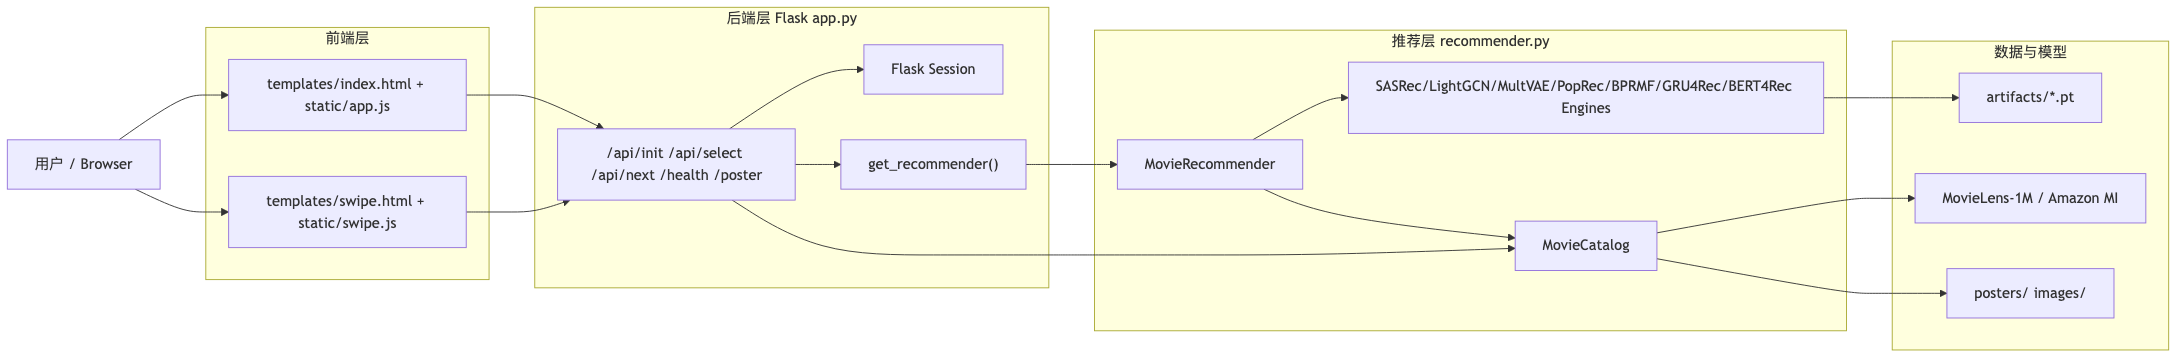
\includegraphics[width=\textwidth,height=0.82\textheight,keepaspectratio]{./diagram_exports/diagram_01.png}
\end{figure}

\section*{2. Module Dependency}
\begin{figure}[H]
  \centering
  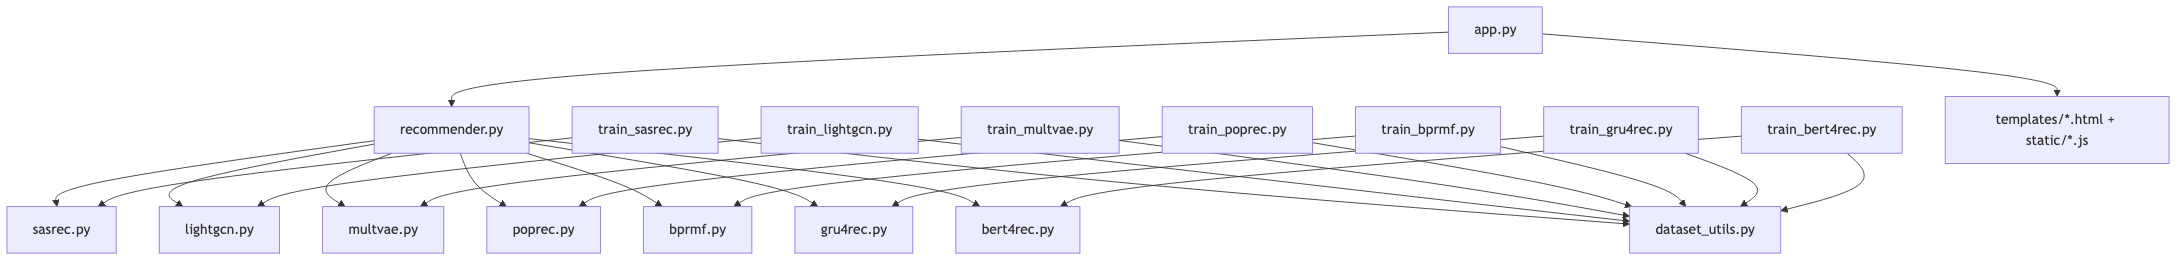
\includegraphics[width=\textwidth,height=0.82\textheight,keepaspectratio]{./diagram_exports/diagram_02.png}
\end{figure}

\section*{3. Core API Sequence (/api/select)}
\begin{figure}[H]
  \centering
  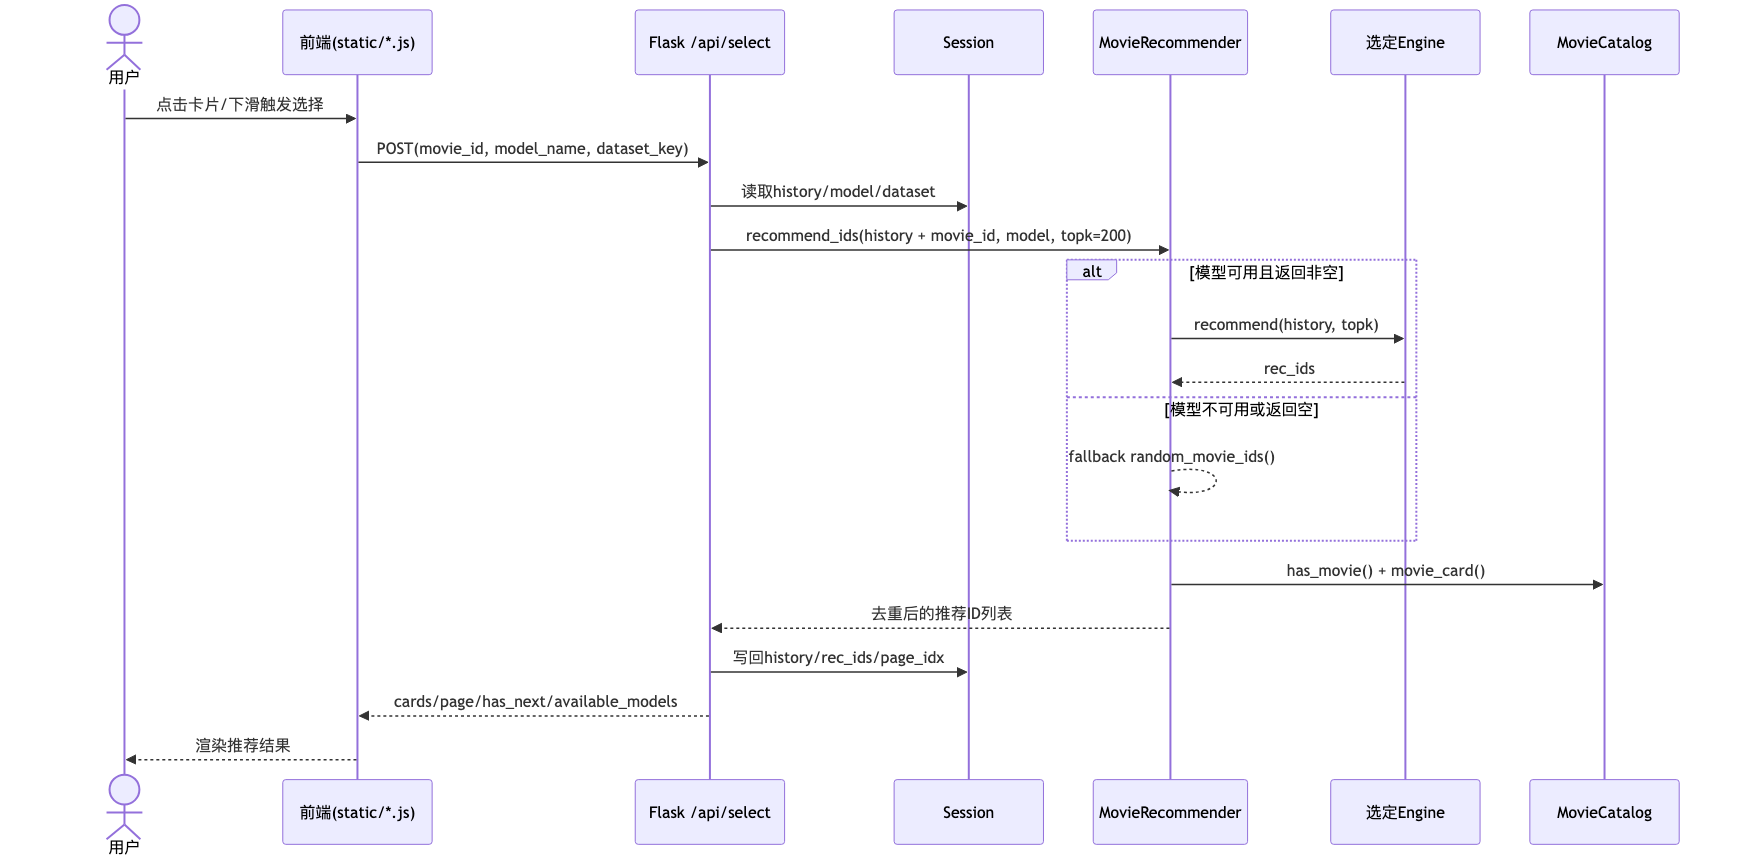
\includegraphics[width=\textwidth,height=0.82\textheight,keepaspectratio]{./diagram_exports/diagram_03.png}
\end{figure}

\section*{4. Training Activity Flow}
\begin{figure}[H]
  \centering
  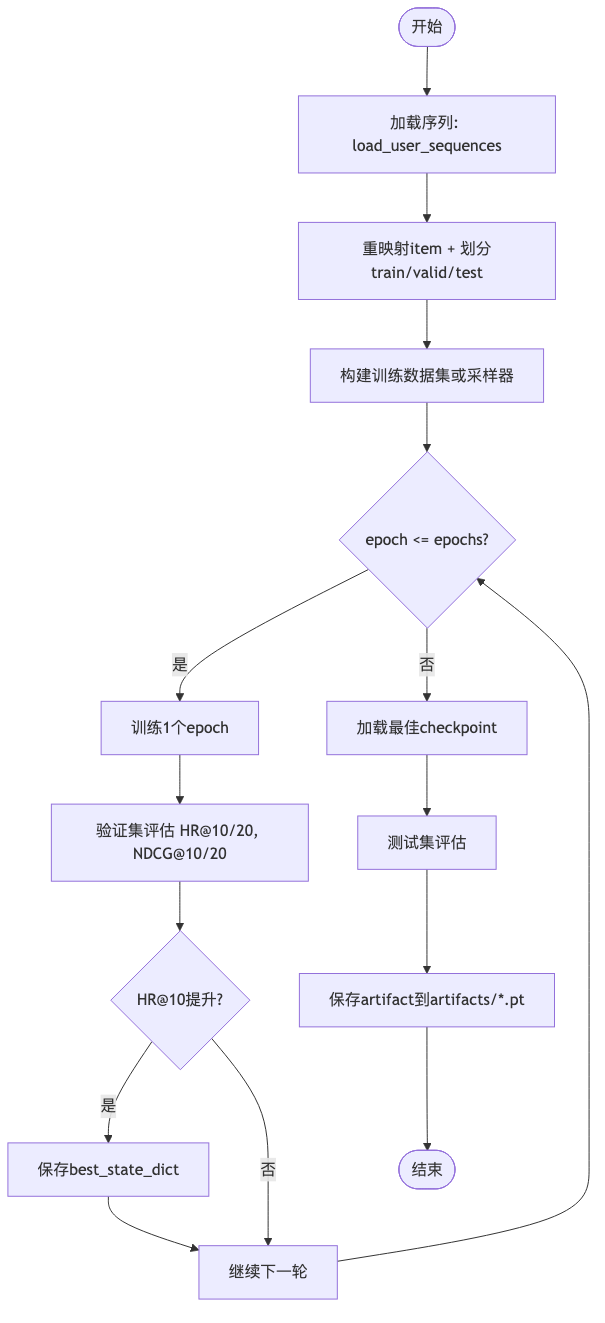
\includegraphics[width=\textwidth,height=0.82\textheight,keepaspectratio]{./diagram_exports/diagram_04.png}
\end{figure}

\section*{5. Session State Machine}
\begin{figure}[H]
  \centering
  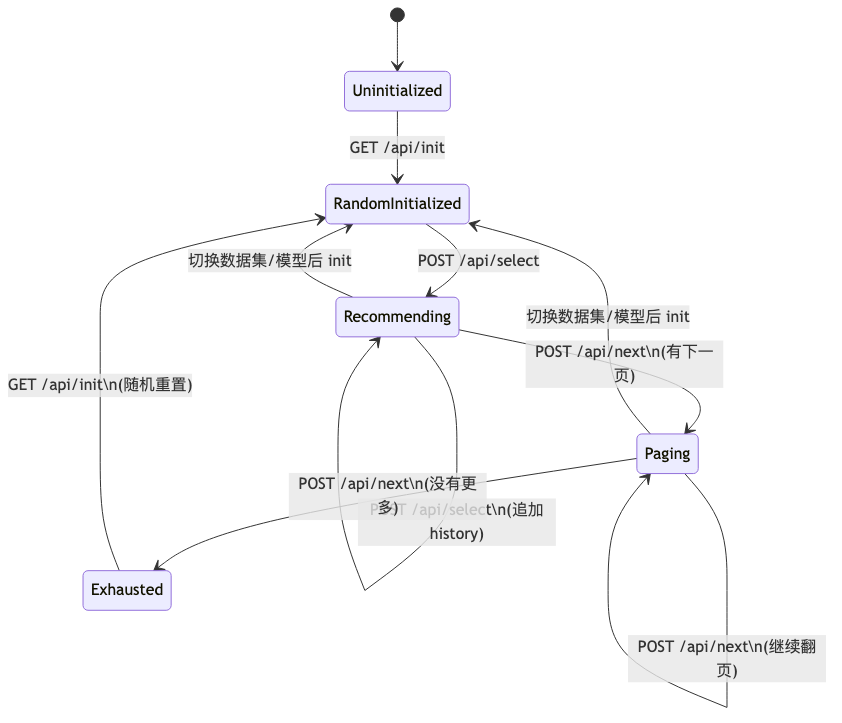
\includegraphics[width=\textwidth,height=0.82\textheight,keepaspectratio]{./diagram_exports/diagram_05.png}
\end{figure}

\section*{6. Deployment / Runtime}
\begin{figure}[H]
  \centering
  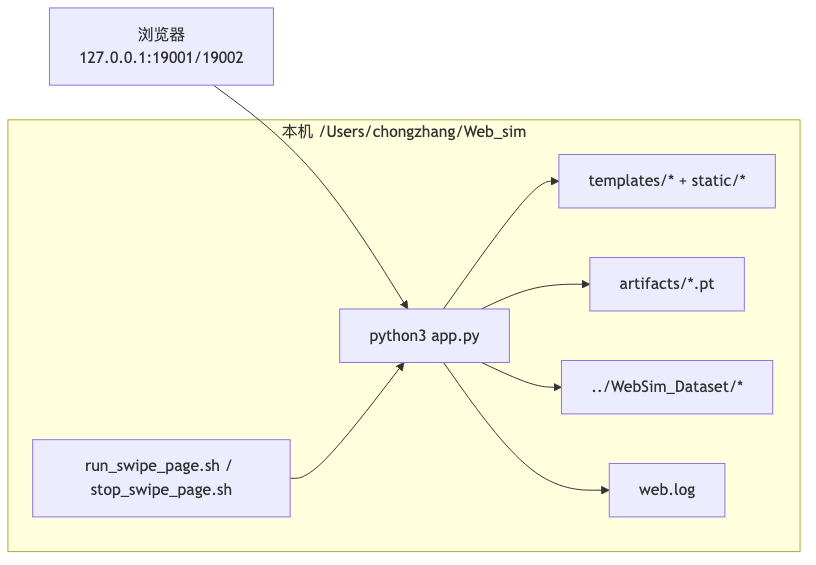
\includegraphics[width=\textwidth,height=0.82\textheight,keepaspectratio]{./diagram_exports/diagram_06.png}
\end{figure}

\end{document}
